% !TEX root = ../main.tex
\section*{3}
\subsection*{a}

This classification problem will be solved by a randomized incremental algorithm, by first shuffling the points randomly and initially choosing two points of different classes 
($P_1$ and $P_2$). The line that passes through both of them will be our initial separating line $l$. \\
\\
As the question is whether there is a line $l$ with the points of $P_1$ above or on it, and the points of $P_2$ below or on it, we can assume that the correct position of points from $P_1$ is above $l$, and the correct position of points from $P_2$ is below $l$.\\
\\
For each of the next points, we check whether it is in the correct position or not. If not, we modify the line $l$. The detailed algorithms is as follows. \\
\\
\\
\textbf{Algorithm:}\\
\\
$FindSeparatingLine$($S$):
\begin{enumerate}
\item Given: Set $S$ of $m$ points of class $P_1$ and $n$ point of class $P_2$  
\item Output: Separating line ( it contains 2 points of different classes) if any or "Not Found"

\item Initialize empty array $Z$
\item S $\leftarrow$ RandomPermutation(S) 
\item Initialize $l$ our initial separating line to be the line between 2 different random points of $P_1$ and $P_2$
\item For every other point  $p  \in S$:
\begin{enumerate}
    \item insert $p$ to $Z$
\item If $p$ is in the proper position
\begin{enumerate}
\item continue 
\end{enumerate}
\item Else  
   \begin{enumerate}
\item $l$  $\leftarrow$ create a new line between $p$ and the point of different class in $l$ 
\item loop on every point in the other class, connect $p$ to the new point if that point is not in the correct position
\item loop on every point in $Z$, if there is a point that not in the proper position, return "Not Found"

\end{enumerate}    
        
\end{enumerate}

\item return $l$
\end{enumerate}

\subsubsection*{Correctness}
We prove the algorithm by induction. \\ 

Based on our selection, the classifier $l$ always contains 1 point from $P_1$ and 1 point from $P_2$. \\

If the dataset contains only one point in $P_1$ and one point in $P_2$, then the algorithm pick the line $l$ passing these points to be the classifier, and this is the correct one. \\

Assume that after processing point $i$, the algorithm has already had the correct solution. Let $p^*$ be the next point, $p_i$ is the point of the same class and $p_i'$ is the point of the different class ($P_1$ or $P_2$) which are 
currently on $l$. When we insert $p^*$, the new classifier should group it to the correct group. \\

If $p^*$ is in the correct order already (the point of $P_1$ should be above or on $l$, and the point of $P_2$ should be below or on $l$), then the classifier $l$ is correct and
the algorithm does not do anything. \\

If $p^*$ is not in the correct order, which means it is on the ``outer'' space of the group of $p_i$, the line $l$ should be modified to group $p^*$ to the proper position. Our algorithm decides to rotate the line $l$ so that it contains $p^*$. This is a proper position for $p^*$ because every point can be on $l$, and $p_i$ is also in that group because $l$ was rotated to the ``outer'' direction. Since the old $l = p_i p_i'$ was the correct classifier, this guarantees that the new line $l = p^* p_i'$ correctly classifies the class of $p^*$. \\ 

After correcting the position of $p^*$, there can be a case that some points of the opposite class are wrong positioned, as being shown in figure \ref{fig:modification}. The algorithm has to perform a loop on the opposite class to correct those points. After this correction, all points of the opposite class are in the right place. The line $l$ can be changed to $p^* p_i''$ where $p_i''$ is the point that better classifies the opposite class. \\

If after that, there are still points outside of their correct positions, which means there are (again) some points in the class of $p^*$ that are in wrong places, then we know that there are no agreements in this case. Thus, there are no line classifiers available for this setting. The algorithm indeed returns false. \\

If all of the points are correctly positioned, then $l$ is obviously the correct classifier. 
So, if the previous step is correct, then the current step is also correct. This implies that our incremental approach is correct. \\

\begin{figure}[h]
\centering
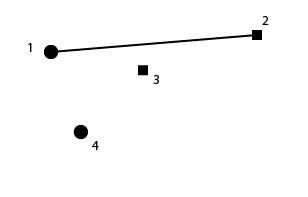
\includegraphics[width=0.5\textwidth]{modification}\\
\caption{Example of 2-round modification. Circles: $P_1$, Squares: $P_2$. 
Intitially, $p_3$ is in the correct order, but after checking $p_4$, we rotate the line to $p_4 p_2$ so that $P_1$ is above the line. So $p_3$ is not correct. Then we have to loop on $P_2$ to put $p_3$ back to the proper position. The final result is $p_4 p_3$.}
\label{fig:modification}
\end{figure}

\subsubsection*{Running Time}
In order to shuffle all points of $P$, the algorithm takes $O(n+m)$.\\

The 2-round check has to traverse the previous processed points for checking correctness, this process takes $O(i)$ where $i$ is the number of points which have been processed. Hence, the expected running time is :
$$
O(n+m) + \sum_{i=1}^{m+n}{ ( Pr[\,p_i \in \text{ProperPosition}\,]*O(1)
    + Pr[\,p_i \not\in \text{ProperPosition}\,]*O(i)
) }
$$

We know that $Pr[\,p_i \in \text{ProperPosition}\,] \le$ 1 and $Pr[\,p_i \not\in \text{ProperPosition}\,]$
is never greater than the probability of selecting 2 points from $i$ points. Thus,
we have :

$$
Pr[\,p_i \not\in \text{ProperPosition}\,] \le 2/i
$$

Hence,
\begin{align*}
T(n+m) &= O(n+m) + \sum_{i=1}^{n+m}( O(1) + O(2/i)O(i) ) \\
&= O(n+m)
\end{align*}

\subsection*{(b)}
The worst case is when the algorithm has to determine $l$ every time processing a
new point. Then, the running time will become $O(n^2)$. \\

Let's consider the case that we perform shuffling on $P_2$ which only takes $O(n)$.
The algorithm takes $O(m)$ to find the first separating line between all points in $P_1$
and one point of $P_2$. Then, for iterating the other points of $P_2$, the running
time when the algorithm has to find a better separating line changes sligthly to
$O(m+i)$, where $i$ is the number of processed points in $P_2$ so far. Hence, the expected running time is :

\begin{align*}
T(n+m) \quad =\quad & O(n) + O(m) \\
        &+ \sum_{i=1}^{n}{ Pr[\,p_i \in \text{ProperPosition}\,]*O(1) } \\
        &+ \sum_{i=1}^{n}{ Pr[\,p_i \not\in \text{ProperPosition}\,]*O(m+i) }
\end{align*}

Hence,

\begin{align*}
T(n+m) &= O(n) + O(m) + \sum_{i=1}^{n}(O(1) + O(2/i)O(m+i)) \\
&= O(m) + 3O(n) + O(m)\sum_{i=1}^{n}1/i \\
&= O(m) + 3O(n) + O(m)O(\ln{n}) \\
&= O(m) + 3O(n) + O(m)O(\log{n}) \\
&= O(m\log{n})
\end{align*}

We can conclude that if we shuffle only some subset of data, in this case only $P_2$,
the algorithm would perform worse.
